
\chapter{Introduction}

\section{History of infectious disease}

Infectious diseases have a profound impact on humankind, influencing the course of wars and the fate of nations. Only two centuries ago, infectious diseases were a defining challenge of the human condition. For perspective, consider that George Washington was born in 1732, a time when there was no well-defined concept of infection or immunity, no vaccines, and not effective treatments for infectious diseases. Washinton suffered from smallpox and malaria, wound infections and abscesses, and nursed his brother on a tropical island as he died of tuberculosis \cite{Fauci:2012us}. Almost all the major advances in the understanding and control of infectious diseases occurred in the two centuries since the founding of the United States. 

Advances began with the first animal-transmission studies conducted soon after the War of 1812. These were followed by the development and improvement of microscopes, which for the first time linked micro-organisms to skin and mucosal diseases. Robert Koch developed unifying principles for infectious disease in the late 1800s, providing criteria to establish a causal link between micro-organism and disease. In the early 20\text{th} century, Paul Ehrlich developed anti-infective serums to kill pathogens, which paved the way for the vaccines, antibiotics, and antiviral agents that saved hundreds of millions of lives and extended the human life span.

\section{Technology}

\subsection{Historical perspective}

Since the seminal contributions of scientists like Koch and Ehrlich, technology has improved our understanding of infectious disease. Though a cornerstone of microbiology since the nineteenth century, culture fails to cultivate or distinguish many microbes. By 1980, only 1800 validated bacterial species had been published \cite{Fournier:2013ewa}. DNA-based analyses changed the paradigm, as they enabled identification and taxonomic classification of micro-organisms based on genetic material (DNA or RNA). 

Hantavirus pulmonary syndrome, an ancient disease caused by a phlebovirus, was discovered unexpectedly in 1993 by the application of a powerful DNA-based assay, polymerase chain reaction (PCR). Less than a year later, PCR-related subtraction techniques solved a century-old mystery of the cause of Kaposi$'$s sarcoma. Since that time, DNA-based analyses have become cheaper and more effective. They have ushered in an era of rapid micro-organism discovery (Figure ~\ref{fig:Fig1}) \cite{Fournier:2013ewa}.

\begin{figure*}
\center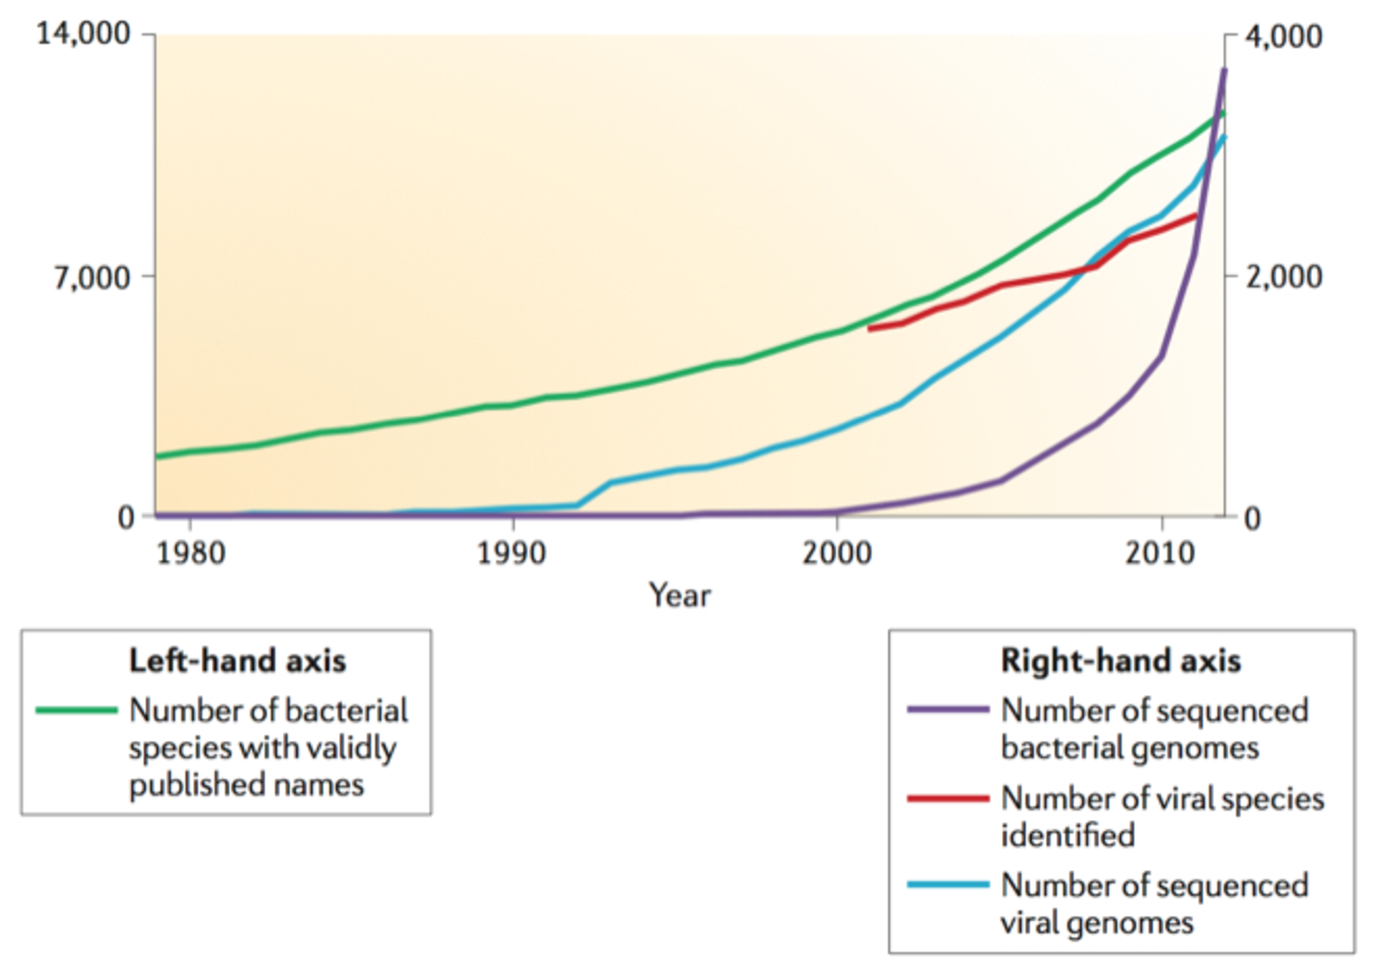
\includegraphics[width=120mm,scale=0.5]{Figures/Fig1}
\caption{Rapid growth in the identification of micro-organisms.}
\label{fig:Fig1}
\end{figure*}

\subsection{Clinical perspective}

Unlike many complex chronic and lifestyle-associated diseases, infectious diseases are usually caused by a single agent. In turn, identification of this agent typically points to disease-control measures (e.g., sanitation) as well as treatment (e.g., vaccination) \cite{Fauci:2012us} and tools to identify agents responsible for a presented infection have been widely sought. The traditional microbiology lab methods for detecting and identifying bacterial pathogens include Gram staining, liquid or solid culture, and the use of the live microbes to assay for antibiotic resistance \cite{Boyd:2013cc}.

Conventional laboratory methods exhibit a trade-off between resolution scope. Culture has favorable scope, meaning that many bacterial pathogens grow in culture and can be identified. However, not all bacterial pathogens can grow in culture. Culture is either not suitable or must be adapted for other pathogens, such as fungi or viruses. As a result, slow-growing, non-bacterial, or exotic pathogens can prove difficult to identify with culture. Furthermore, resolution may be poor, meaning that there may be - for example - no way to distinguish between strain or species with culture. On the other hand, DNA-based methods such as qPCR have high resolution. They typically can identify a single micro-organism at high (e.g., strain or species) resolution. Yet, the assay works only for a single micro-organism.

\begin{figure*}
\center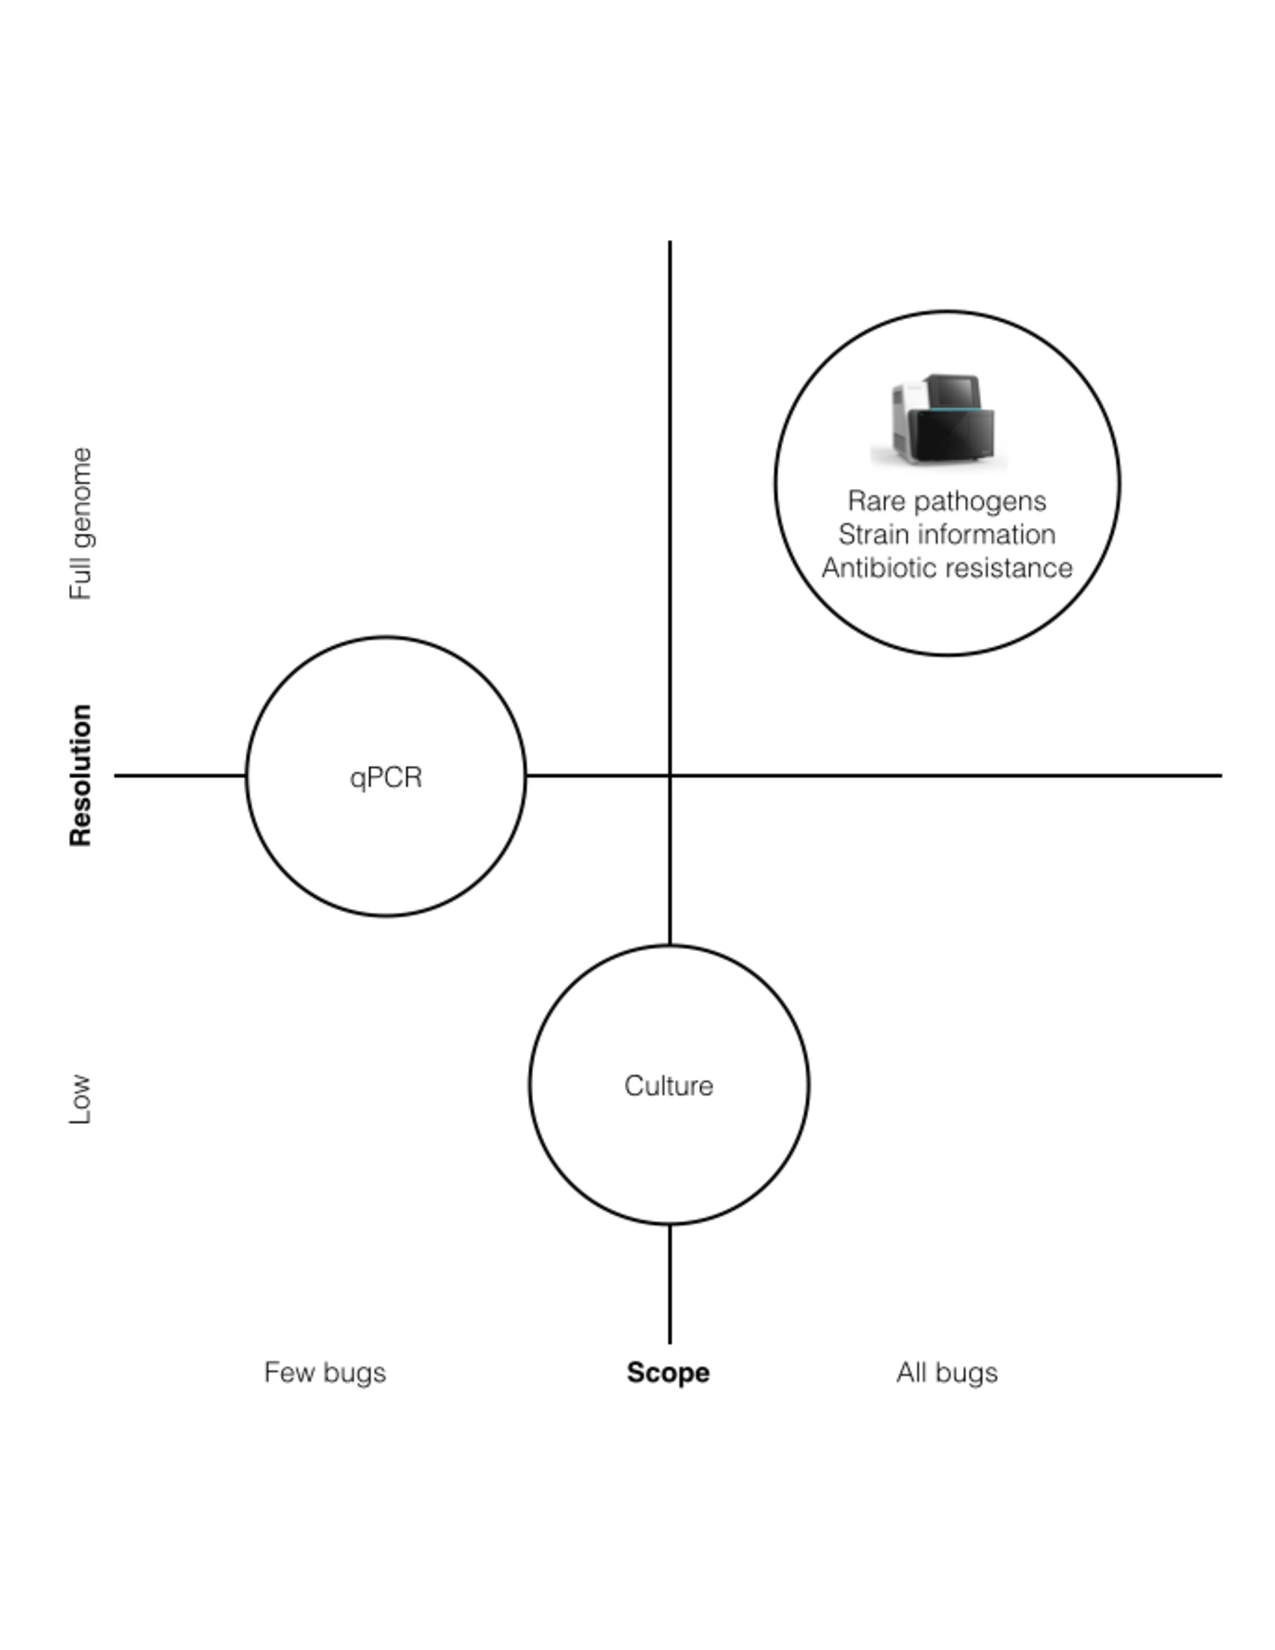
\includegraphics[width=125mm,scale=0.5]{Figures/Fig2}
\caption{The trade-off between scope and resolution.}
\label{fig:Fig2}
\end{figure*}

\subsection{High-throughput methods}

Some consider that the rapid identification of the SARS virus in 2003 ushered in a new era of pathogen identification. This was achieved through a combination of high-throughput techniques (nucleic acid microarray hybridization) and traditional viral culture and real-time PCR \cite{Boyd:2013cc}. Since that time, high-throughput techniques, such as MALDI-TOF mass spectrometers, have become gradually introduced to clinical workflows. By comparing protein signature in a clinical sample with a collection of patterns that have been deposited in a database, MALDI-TOF can often achieve better resolution and faster turn-around time than culture \cite{Fox:2014fj}. Yet, the discriminatory power of the method varies depending on the target micro-organism as well as the database used. Some bacteria are under-represented in MALDI-TOF databases, technical problems (e.g., variations in culture or sample preparation) can affect the discriminatory power, and many commercial databases do not include viruses. 

Soon after the publication of the Sanger-sequenced human genome draft results in 2001 and the "finished" sequence in 2004, several new DNA sequencing technologies were described in the literature. Most used a flow-cell surface or beads in an emulsion to spatially segregate individual DNA template molecules so that they can be amplified \emph{in situ} and sequenced in parallel with simultaneous data acquisition from millions of templates via optical or electronic detection \cite{Boyd:2013cc}.

These technologies ushered in an era of next-generation DNA sequencing (NGS). As costs drop and performance improves, NGS is becoming an appealing alternative (or supplement) to MALDI-TOF, culture, or targeted DNA-based methods like qPCR \cite{Shendure:2012et}. The critical advantage of NGS in for infectious diseases is that it can, in principle, assay every gene and every conceivable marker derived from infectious agents in a sample. Whereas MALDI-TOF relies on a handful of signature proteins, NGS is capable of identifying an unlimited set of possible pathogens (unlimited scope) as well as the complete genomic sequence of each one (high resolution) (Figure ~\ref{fig:Fig2}). With sufficiently long read lengths, multiple reads mapping to a specific microbial genomes, and a well-annotated reference database, nearly all microorganisms can be uniquely identified on the basis of their nucleic acid sequence  \cite{Boyd:2013cc}.

\subsection{The case for high-throughput sequencing}

There are two central reasons driving interesting in unbiased NGS for comprehensive detection of pathogens from clinical samples: (1) Conventional diagnostic testing for pathogens still fails to detect the causal agent in a significant percentage of cases \cite{Naccache:2014gk}. (2) Failure to accurately diagnose and treat infection in a timely fashion contributes to continued transmission and increased mortality in hospitalized patients. Furthermore, a rising tide of studies have collectively made a strong case for the introduction of NGS into the clinic for various compelling scenarios.

\textbf{Unbiased screening of rare pathogens}: Because NGS performs unbiased measurement of all nucleic acids in a clinical sample, it can reveal pathogens that escape conventional clinical testing. A recent study applied NGS to a 14-year-old boy with severe immunodeficiency who presented with fever and headache that gradually progressed to hydrocephalus and status epilepticus \cite{Wilson:2014dv}. Conventional diagnostic workup, including brain biopsy, was unrevealing. Yet, unbiased next-generation sequencing of the cerebrospinal fluid identified \emph{Leptospira}, an exotic pathogenic bacteria. Though conventional clinical assays for leptospirosis were negative, detection with NGS informed intervention and allowed the patient to make a full recovery. 

\textbf{Outbreaks}: Microbiologists and physicians often need to look broadly before determining the virulence genes in a particular strain account for an outbreak. NGS facilitates this search. For example, NGS was used to identify a novel strain of \emph{Escherichia coli}, O157, during a food-borne outbreak in Germany \cite{Fox:2014fj}. Similarly, NGS has been applied to the US epidemic of community-associated methicillin-resistant Staphylococcus aureus (MRSA). NGS indicated that most strains were very closely related across geographical locales, implicating expansion from a single population rather than convergent evolution of different strains \cite{Boyd:2013cc}. As a finally example, NGS applied to the Haitian cholera outbreaks traced its probable origin to UN solders that inadvertently brought the infection from Bangladesh \cite{Boyd:2013cc}.

\textbf{Resistance}: NGS cam be used to determine whether plasmids or other mobile genetic elements carrying antimicrobial drug-resistance genes are being transferred among the bacterial pathogens infecting patients. For example, the NIH recently experienced an outbreak of carbapenem-resistant \emph{K. pneumoniae} that affected 18 patients and killed 11. Integrated genomic and epidemiological analysis traced the outbreak to three independent transmissions from a single patient who was discharged 3 weeks before the next case became clinically apparent and pointed to possible explanations for these transmissions \cite{Fox:2014fj}. Similarly, NGS applied to patients infected with HIV has been used to reveal viral subpopulations and low-frequency mutant viral strains with antiviral resistance?associated sequence changes \cite{Boyd:2013cc}.

\textbf{Culture-free}: NGS is valuable in clinical settings when dealing with difficult-to-culture or notoriously slow-growing pathogens such as \emph{Mycobacterium tuberculosis}.

\textbf{Microbial populations}: NGS can be used to explore microbial diversity and full populations. Nine Mycobacterium species can cause tuberculosis. Some strains, such as \emph{Mycobacterium bovis}, require specific antibiotic treatments, making high resolution NGS particularly valuable \cite{Fox:2014fj}. Furthermore, the human microbiome project has highlight the importance of assaying microbial populations \cite{Consortium:2012bb}. Community-wide profiling and examination of changes in relative abundance may become increasingly important as we learn more about human microbiology.

\subsection{NGS challenges and opportunities}

\textbf{Cost and speed}: The cost and turn-around time for sequencing have both been driven down by hardware advances. The cost for determining individual microbial genomes continue to fall and costs as little as \$100 per sequence \cite{Fox:2014fj} with multi-hour turn-around. Both will continue to improve and the justification for NGS will become increasingly apparent, starting with hospital patients who develop difficult-to-treat or life-threatening infections that prove very costly to the system.

\textbf{Informatics}: NGS technology produces large datasets that require extensive bioinformatics simply for sequence analysis. Data presentation and distillation of clinical recommendations from large datasets also prove challenging. Addressing informatic challenges associated with NGS will be critical for widespread adoption.
 
\textbf{Mechanism}: Increasingly, NGS has been applied to the molecular networks that underlie cells, including chromatin immunoprecipitation with subsequent high-throughput sequence analysis (ChIP-Seq) for protein-DNA interactions, high-throughput RNA sequencing (RNA-Seq) for transcription, Ribo-Seq for translation, parallel analysis of RNA structure (PARS) for structure assays, and global mapping of DNA-DNA interactions using proximity ligation coupled with deep sequencing (Hi-C) \cite{Shendure:2012et}. Many of these methods could also be applied to the study infectious disease. 

\section{Contributions and outline of this thesis}

\subsection{Molecular counting for diagnostics}

In this thesis, we show that molecular counting of pathogen-derived cell-free DNA is a powerful diagnostic. We built a pipeline for counting pathogen-derived cell-free molecules in human plasma and a web application presenting the resulting data. We applied these tools to thousands of clinical samples collected from hundreds of patients at Stanford hospital. We further processed thousands of clinical test records in order to show that this method can be broadly applied for non-invasive monitoring of viral, bacterial, and fungal infections in deep tissues. Finally, we show that unbiased pathogen monitoring using this technique can track rare or un-expected infections that now escape hypothesis-centric clinical testing.
   
\subsection{Molecular counting for mechanism}

After demonstrating this new diagnostic application of NGS, we show how NGS technology can be used to understand infectious disease mechanism. We developed a pipeline for counting of sequencing reads derived from RNA-protein interactions \emph{in vivo}. We show that this method (CLIP-seq) can be applied to viruses that have infected human cells and use it to reveal novel interactions between the HCV genome and human protein PCBP2. In a follow-up study, we applied the method to HERV-K, an endogenous retrovirus. We showed that human embryo development occurs in the presence of retroviral products, which protect the embroyo from exogenous infection while exerting regulatory function through interaction with human mRNAs. 

We highlight three separate ways to validate results from mechanistic CLIP-seq experiments, including comparative analysis, replicate matching, and functional studies. We also developed a highly multiplexed RNA-protein interaction assay that is compatible with the scale of CLIP-seq experiments and far exceeds the throughput of common biochemical assays. We applied this technology to a model RNA-protein interaction (histone stem-loop and SLBP), recapitulating two decades of biochemistry in a single experiment while also revealing novel features of the interaction.  